\documentclass[12pt]{article}
\usepackage{listings}
\usepackage{url}
\usepackage{placeins}
\usepackage[paper=letterpaper,
           marginparwidth=1in,
           hmargin={1.1in,0in},
           vmargin={1in,1.5in},           
           includemp
           ]{geometry}
           
 \usepackage{longtable}
 \usepackage{graphicx}
 \usepackage{caption}
\usepackage{subcaption}
\usepackage[]{natbib}
\usepackage{latexsym,amsfonts,amssymb,amsmath,amsthm,mathrsfs}
\usepackage{bbm}
\usepackage{amsthm}
\newtheorem{definition}{Definition}
\usepackage{hyperref}
\usepackage{lscape}

\hypersetup{
    bookmarks=true,         % show bookmarks bar?
    unicode=false,          % non-Latin characters in Acrobat’s bookmarks
    pdftoolbar=true,        % show Acrobat’s toolbar?
    pdfmenubar=true,        % show Acrobat’s menu?
    pdffitwindow=false,     % window fit to page when opened
    pdfstartview={FitH},    % fits the width of the page to the window
    pdftitle={My title},    % title
    pdfauthor={Author},     % author
    pdfsubject={Subject},   % subject of the document
    pdfcreator={Creator},   % creator of the document
    pdfproducer={Producer}, % producer of the document
    pdfkeywords={keyword1} {key2} {key3}, % list of keywords
    pdfnewwindow=true,      % links in new window
    colorlinks=true,       % false: boxed links; true: colored links
    linkcolor=red,          % color of internal links (change box color with linkbordercolor)
    citecolor=black,        % color of links to bibliography
    filecolor=magenta,      % color of file links
    urlcolor=blue           % color of external links
}
\providecommand{\keywords}[1]{\textbf{\textit{Keywords ---}} #1}


\begin{document}
\title{Final Project: Implementation of PSRL and UCRL in the RLPy platform}
\date{March 18, 2015}
\author{Imanol Arrieta Ibarra}
\maketitle

\begin{abstract}
RLPy is a python library that implements several Reinforcement Learning algorithms in an object-oriented environment. By incorporating UCRL and PSRL to this platform I am able to easily compare these algorithms across a great gamma of already implemented domains. In the following document I will compare PSRL, UCRL, SARSA and LSPI across two domains. The first is a classic MDP chain problem and the second one is the solution of a labyrinth. 
\end{abstract}

\section{MDP Chain}

This experiment consists of a chain of 10 nodes. The agent starts in the first node and has to reach the 10th in order to get a reward of 1.  Figure \ref{fig:res_mdp} shows how the different algorithms performed on this domain. Each line is the average over 5 different runs, the shadow area around the line represents the confidence interval. The graph is a little misleading,  because of the exploring in PSRL and UCRL, the average of multiple runs will be lower than the optimum. If we were to take a single run of each algorithm all would typically 
end up converging to the optimum. 

\begin{figure}[h]
\centering
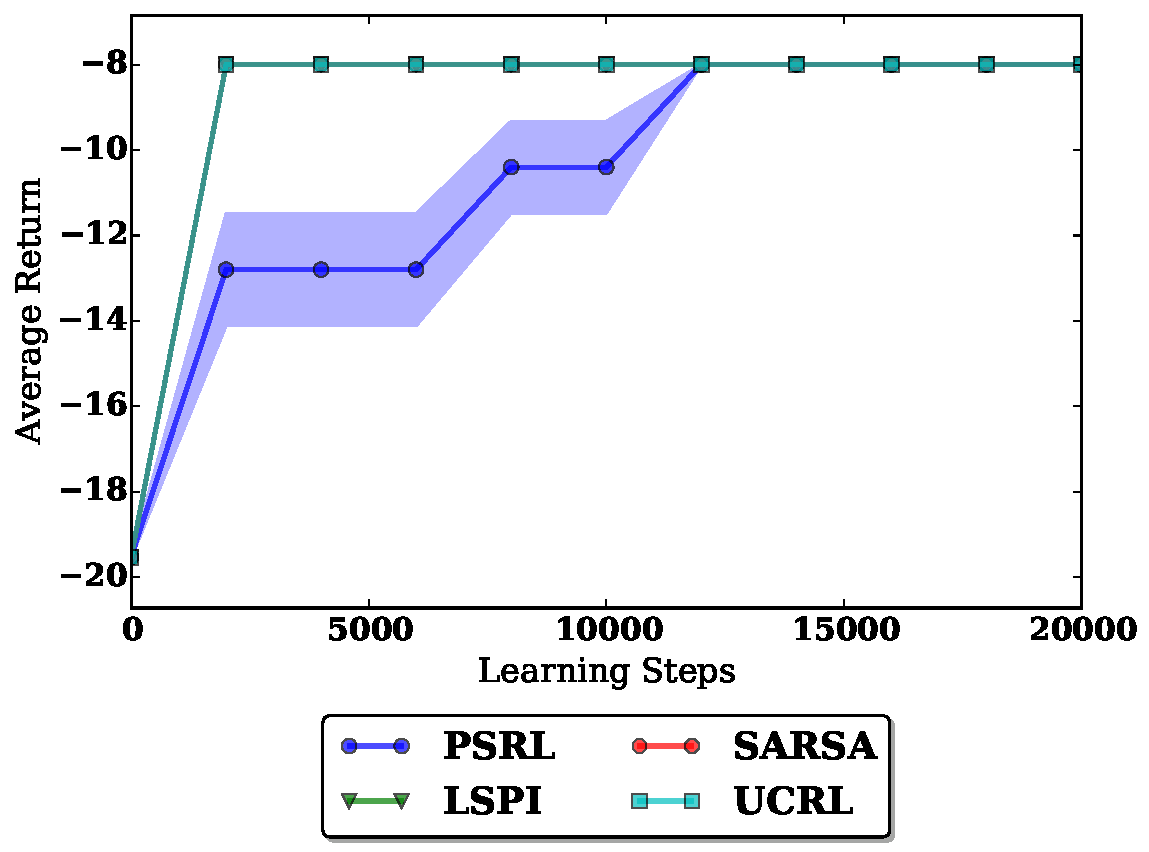
\includegraphics[scale=.4]{MDP.pdf}
\caption{Average Return for the MDP chain}
\label{fig:res_mdp}
\end{figure}


\FloatBarrier
\section{GridWorld}
This experiment consists on a labyrinth with two pits and a way out. The starts at the beginning of the labyrinth and moves until the number of steps is maximum, it encounters a pit or it reaches the end. Figure \ref{fig:GW} shows how the labyrinth looks like. The blue square corresponds to the starting point, the red ones to the pits, the gray ones to the walls and the green one to the exit.

\begin{figure}[h]
\centering
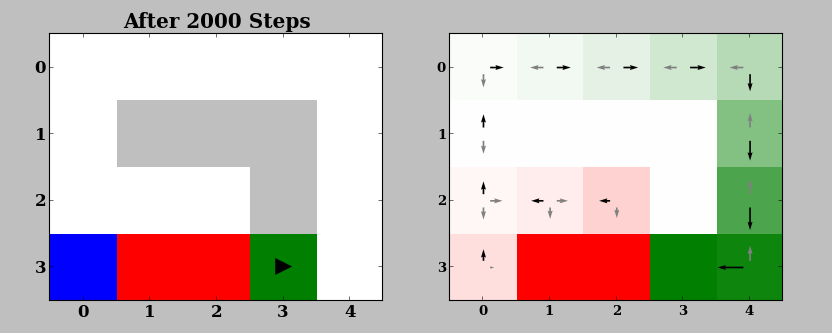
\includegraphics[trim=0cm 0cm 0cm 1.1cm, clip=true, scale=.4]{gridWorld.png}
\caption{GridWorld labyrinth and example of policy}
\label{fig:GW}
\end{figure}

The adaptation of UCRL and PSRL to this setting was tricky because of the way RLPy is designed. I had to use some hacks in order to translate what the platform intended to do and what PSRL and UCRL need as input. Both UCRL and PSRL look pretty unstable in figure \ref{fig:res_grid}. This has to do in part with the stochasticity of the GridWorld problem

\begin{figure}[h]
\centering
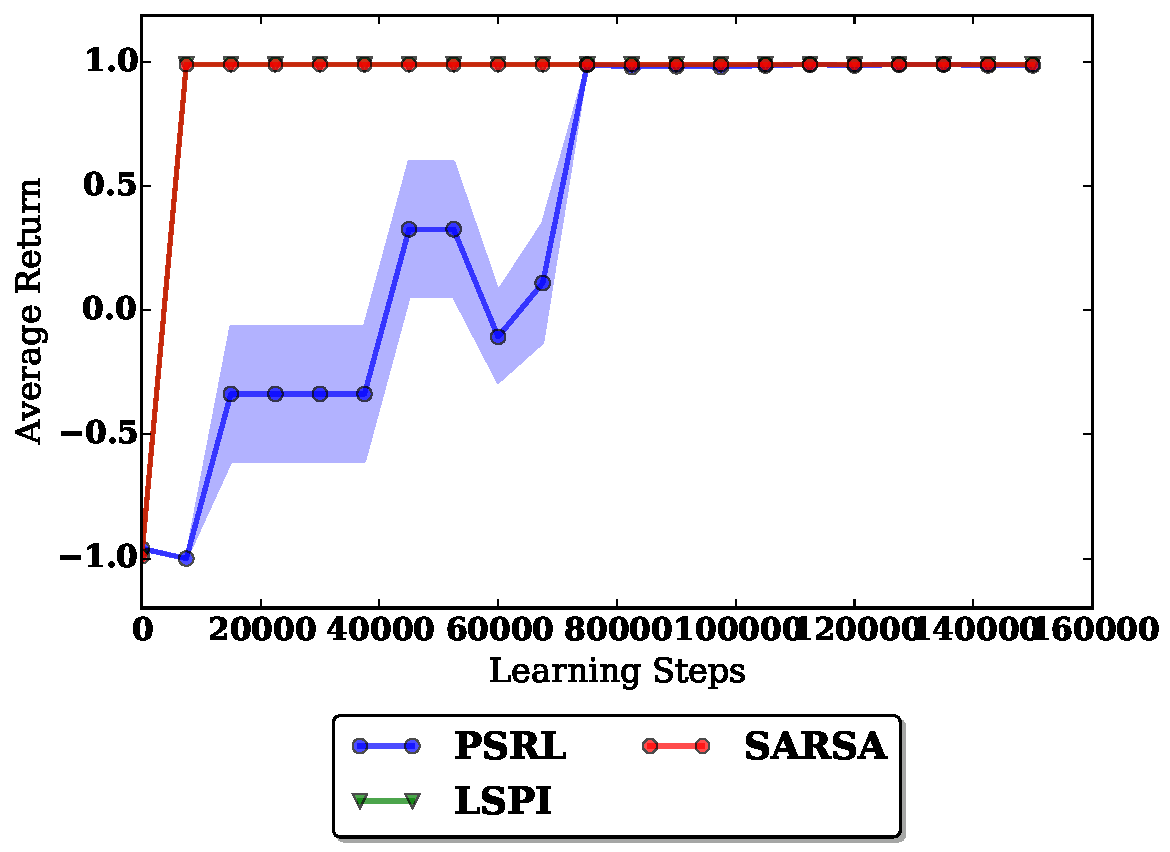
\includegraphics[scale=.4]{Grid.pdf}
\caption{Average Return for GridWorld}
\label{fig:res_grid}
\end{figure}

\section{Code}
The code for this project can be found in \url{https://github.com/imanolarrieta/RL.git}. The files are located in: rlpy/Agents/UCRL and rlpy/Agents/PosteriorSampling.

\section{Conclusions}
These are some of the examples in which we would be able to test PSRL and UCRL. The only disadvantage and the reason I am not presenting any more is that because of Python limitations, the implementation of PSRL and UCRL can not be properly vectorized and as such runs extremely slow. However, if time is not a constraint, having this two algorithms in this platform provides great opportunity to compare them to Q-learning type algorithms.
\newpage

\bibliographystyle{chicago}
\bibliography{biblio}



\end{document}